Since web service API and  Database are hosted on Cloud service, no hardware is required. This section will discuss API tool platforms and databases.

\subsection{Web Service API}
API is an application interface that integrates two applications or systems to support the transfer of data to each other. Mulesoft is a platform where provides many convenient functions to build and deploy API. Using Mulesoft make it easier to connect MySQL.

\begin{figure}[h!]
	\centering
 	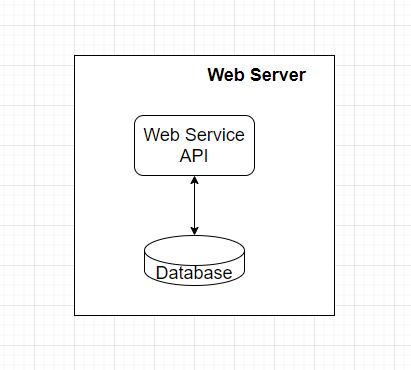
\includegraphics[width=0.60\textwidth]{images/web_layer.PNG}
 \caption{Example subsystem description diagram}
\end{figure}

\subsubsection{Web Service API Software Dependencies}
MuleSoft Exchange provides many dependencies and other APIs that are needed to build our API through a connector that prebuilds connectivity to an endpoint. 

\subsubsection{Web Service API Programming Languages}
DataWeave is the MuleSoft expression language for accessing and transforming data that travels through a Mule app. 

\subsubsection{Web Service API Data Structures}
MuleSoft Design Center has a function called API specification which helps to define incoming and output data format and creates automated documentation for the APIs. Through API specification, the general structure of API will be provided.

\subsubsection{Web Service API Data Processing}
API will listen to HTTP requests and based on a certain path, it will retrieve data from the database and return it to the user. 


\subsection{Database}
The online database allows you to store sensor readings from the ESP32 and read from anywhere in the world by accessing your server domain.
\subsubsection{Database Programming Languages}
A query is used to communicate with the database. 

\subsubsection{Database Data Structures}
There are some required tables that the database has to have such as temperature for each component and recipe. 

\subsubsection{Database Data Processing}

The database will Run the query for requests and return the data to API.
